\documentclass[10pt]{article}\usepackage[margin=.65in]{geometry}\usepackage[T1]{fontenc}\usepackage{graphicx}\setlength{\parindent}{0pt}\setlength{\parskip}{7pt}\sloppy\begin{document}{\large Native independent matrix verification}\par The native replacement recomputes all 105 ordered matrix identities and normalized roots across the 21 retained models. Its outputs agree exactly with the original native producer result. Ten native fixed controls pass, and two actual CLI corruption controls reject a substituted walk source and an altered binding manifest with exit1. Final replay is byte-identical.\par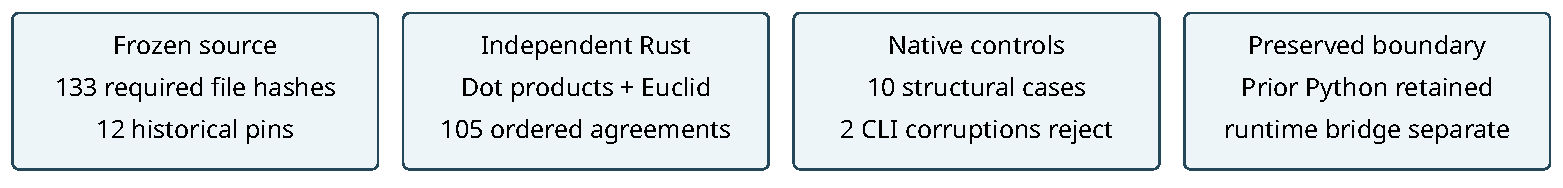
\includegraphics[width=\linewidth]{diagram.pdf}\par Repository-rule correction. The preceding independent recompute.py and its control driver were Python research verifiers, contrary to AGENTS.md. Their published evidence remains unchanged. This packet replaces that execution path with Rust and shell-only build/run orchestration. The original native producer is unchanged. The replacement is a producer packet awaiting independent source-fidelity review after publication.

Arithmetic. The implementation independently forms row-column dot products with u128 sums and computes normalization inverses by extended Euclid, instead of the original producer's Fermat exponentiation. It requires prime p$<$=2\textasciicircum{}32, canonical four-by-four matrices, nonzero canonical scalar certificates, canonical distinct roots, nonzero normalization denominator, exactly21 model keys and exactly5 ordered actions per model. The fixed saved rows agree individually, not merely by an aggregate count.

Custody and acceptance. The checker compiles the SHA256 of the already-published 133-file input-binding manifest. Every file in that snapshot must match before and after the computation. Twelve historical source pins are also checked. Both literal loader/linear section equality and inclusion in the two bound full sources are verified. An altered supplied walk file now fails inside the checker itself; changing the manifest cannot silently approve the substitution. The historical cached and later uncached source versions remain distinct. This is source custody, not an executed collector binary attestation.

Controls. Six structural/algebraic mutations reject wrong shape, noncanonical entry, changed coefficient, missing model, reversed scalar order and zero normalization denominator. A duplicate model rejects; the identity matrix accepts; composite modulus and zero scalar reject. The two CLI controls operate on a private copied snapshot and on an altered manifest, preserve their actual outputs and require nonzero exit. No original input was edited.

Scope. This checks fixed retained coefficients and records, not point enumeration, solver trajectories, timing or geometric action interpretation. The original 1,260-target obligation and expired scientific limits remain unchanged. Native row-fold semantics and actual runtime-input provenance are separate interfaces. A third party can restore the exact pinned producer snapshot and run check.sh; the frozen binding SHA is explicit in src/main.rs.
\end{document}